Here we consider a standard epidemic model to describe the dynamics of a 
disease. We use optimal control techniques to find a vaccination
schedule for the disease. Our goal is to minimize the number of infectious 
persons and the overall cost of the vaccine during a fixed time period. 

Let $S(t)$ be the number of susceptible individuals, $I(t)$ the
number of infectious individuals, and $R(t)$ the recovered (inmune)  at time
$t$. Also, we consider a class that represent the number of exposed or latent
individuals at time $t$, $E(t)$. 
Finally, let $N(t) = S(t) + E(t) + I(t) + R (t)$,
be the total number of people in the population.

Let $u(t)$, the control, be the percentage of susceptible individual being 
vaccinated per unit of time. As vaccination of the entire susceptible population
is impossible, we bound the control with $0 \leq u(t) \leq 0.9$. Let $b$ be the
natural exponential birth rate of the population and $d$ the natural exponential
death rate. 

The optimal control problem is as follows,

$$
    \min_{u} J(u) = \min_{u} \int_{0}^{1} AI(t) + u^{2}(t) dt,
$$
subject to
\begin{align*}
    \dot{S}(t) &=
        bN(t) - dS(t) - cS(t)I(t) - u(t)S(t) \quad, S(0) = S_0 \geq 0,   \\
    \dot{E}(t) &=
        cS(t)I(t) - (e + d)E(t) \quad, E(0) = E_0 \geq 0,    \\
    \dot{I}(t) &=
        eE(t) - (g + a +d)I(t) \quad, I(0) = I_0 \geq 0,     \\
    \dot{R}(t) &=
        gI(t) -dR(t) + u(t)S(t) \quad, R(0) = R_0 \geq 0,    \\
    \dot{N}(t) &=
        (b - d)N(t) - aI(t) \quad, N(0) = N_0 \geq 0,        \\
\end{align*}
where $0 \leq u(t) \leq 0.9$. Note that the disease free state is 
$(bN/d,0,0,0)$.

The Hamiltonian for this problem is
\begin{align*}
    H(t,x,u,\lambda) &= AI + u^{2} + \left< \lambda , g \right> \\
                     &= AI + u^{2} + \sum_{i \in J} \lambda_{i}g_{i}
\end{align*}
where $J = \{S, E, I, R\}$ and $g_i$ is the right hand side of the corresponding
equation.

%---------%---------%---------%---------%---------%---------%---------%---------
\begin{theorem} 
    There exists an optimal control $u^{*}$ and corresponding solutions, \break
    $S^{*}, E^{*}, I^{*}, T^{*}, N^{*}$ that maximizes $J(u)$ over $[0, 1]$. 
    Also, there exists adjoint functions, $\lambda_{i}, i \in J$, such that
    \begin{align*}
         \dot{\lambda}_{S} &=
            \lambda_{S}\left(d + cI + u \right) - \lambda_{E}cI - 
            \lambda_{R}u   \\
        \dot{\lambda}_{E} &=
            \lambda_{E}(e + d) - \lambda_{I}e  \\
        \dot{\lambda}_{I} &=
            (\lambda_{S} - \lambda_{E})cS + \lambda_{I}(g + a +d) - \lambda_{R}g
            \lambda_{N}a\\
        \dot{\lambda}_{R} &=    \lambda_{R}d  \\
        \dot{\lambda}_{R} &=
            - \lambda b - \lambda_{R}d  (b - d)
    \end{align*}
\end{theorem}


\begin{figure}[tbh!]
\centering
	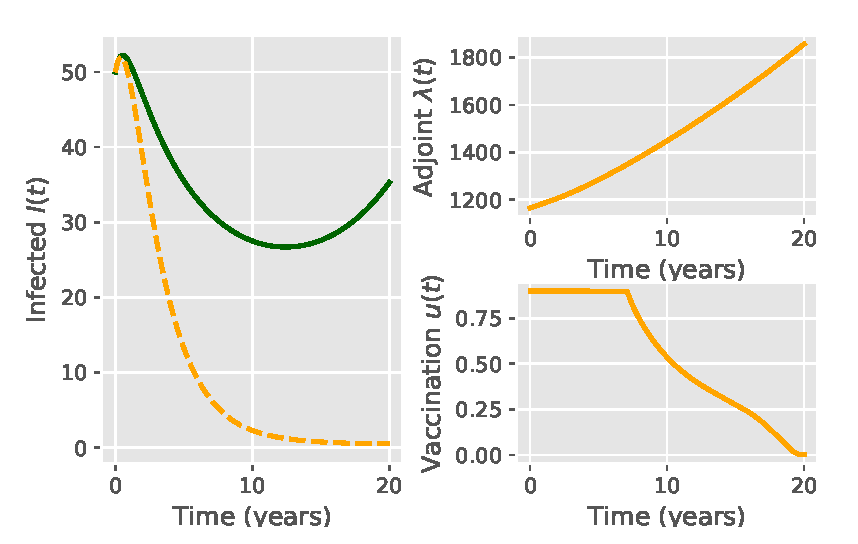
\includegraphics[width=0.7\linewidth]{./Figures/epidemics_lenhart_lab7}
	\caption{Likening between the controled and uncontrolled Infected 
	 population.  At right, we show the optimal infected state agains the 
	 dynamics without 
	 control. At right we present the corresponding adjoint function $\lambda$ 
	 and the optimal control.}
\label{fig:epidemicslenhartlab7}
\end{figure}
